\chapter{Lecture of 04/03/2026}

\begin{example}

    hyperplane $\{ x \in \Rn | \alpha^\top x = b \} a \in \Rn, b \in \R$ 

    halfspaces $\{x \in \Rn| \alpha^\top x \leq b\}$
    
\end{example}

Polyedra $\{x \in \mathbb{R}^n | a_i^\top x \leq b_i \}$ with $a_1, \ldots, a_m \in \mathbb{R}^n, b_1, \ldots, b_m \in \mathbb{R}^n$

C $\subset \Rn$ cone if $\lambda x \in C$ for every $x \in C$ and $\lambda > 0$.
\begin{figure}[ht!]

    \centering
    
 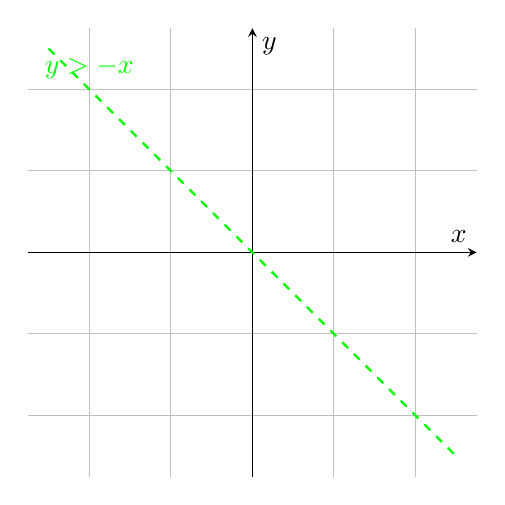
\begin{tikzpicture}
    \begin{axis}[
        axis lines=middle,
        xlabel={$x$},
        ylabel={$y$},
        xmin=-5.5, xmax=5.5,
        ymin=-5.5, ymax=5.5,
        grid=major,
        unit vector ratio=1 1,
        ticks=none
      ]
      \addplot [green, thick, dashed, samples=2] {-x} node [pos=0.1, above] {$y > -x$};
      \addplot [gray!20, draw=none, domain=-5:5, samples=100] {-x+0.1} \closedcycle;
      \addplot [gray!20, draw=none, domain=-5:5, samples=100] {-x} \closedcycle;
      \addplot [gray!20, draw=none, domain=-5:5, samples=100] {-x-0.1} \closedcycle;
    \end{axis}
  \end{tikzpicture}
  \caption{Open cone.}

\end{figure}
\begin{figure}[ht!]

    \centering
    
 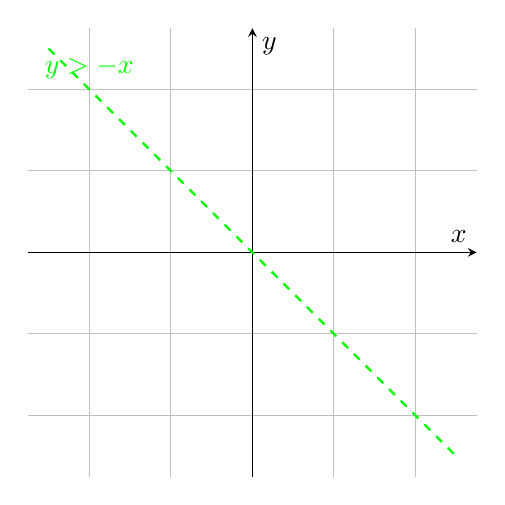
\begin{tikzpicture}
    \begin{axis}[
        axis lines=middle,
        xlabel={$x$},
        ylabel={$y$},
        xmin=-5.5, xmax=5.5,
        ymin=-5.5, ymax=5.5,
        grid=major,
        unit vector ratio=1 1,
        ticks=none
      ]
      \addplot [green, thick, dashed, samples=2] {-x} node [pos=0.1, above] {$y > -x$};
      \addplot [gray!20, draw=none, domain=-5:5, samples=100] {-x+0.1} \closedcycle;
      \addplot [gray!20, draw=none, domain=-5:5, samples=100] {-x} \closedcycle;
      \addplot [gray!20, draw=none, domain=-5:5, samples=100] {-x-0.1} \closedcycle;
    \end{axis}
  \end{tikzpicture}
  \caption{This set is not convex since the line segment connecting two points in the set is not entirely contained in the set.}

\end{figure}
\begin{definition}[Convex function]
    A function $f: \Rn \to \R$ is convex if its domain is a convex set and for all $x, y$ in the domain and all $\theta \in [0, 1]$,
    \[
        f(\theta x + (1 - \theta) y) \leq \theta f(x) + (1 - \theta) f(y).
    \]
\end{definition}
\begin{figure}[ht!]

    \centering
    
 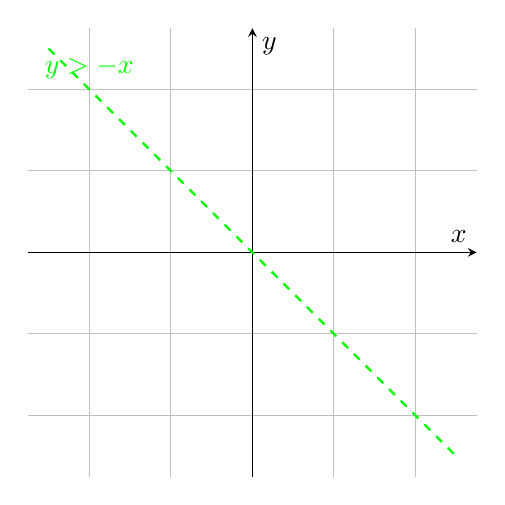
\begin{tikzpicture}
    \begin{axis}[
        axis lines=middle,
        xlabel={$x$},
        ylabel={$y$},
        xmin=-5.5, xmax=5.5,
        ymin=-5.5, ymax=5.5,
        grid=major,
        unit vector ratio=1 1,
        ticks=none
      ]
      \addplot [green, thick, dashed, samples=2] {-x} node [pos=0.1, above] {$y > -x$};
      \addplot [gray!20, draw=none, domain=-5:5, samples=100] {-x+0.1} \closedcycle;
      \addplot [gray!20, draw=none, domain=-5:5, samples=100] {-x} \closedcycle;
      \addplot [gray!20, draw=none, domain=-5:5, samples=100] {-x-0.1} \closedcycle;
    \end{axis}
  \end{tikzpicture}
  \caption{convex function on $\R^2$.}

\end{figure}

f is said to be \textbf{concave} if $-f$ is convex.

\begin{example}

    \[f(x) = a^{\top}x + b \phantom{suca} a \in \Rn, b \in \R \]
    \[f(\gamma x +(1-\gamma)y) = \<a, \gamma x + (1 - \gamma)y \> + b(1 - \gamma + \gamma)\]
    \[  (\langle a, x \rangle + b) +(1- \gamma)(\langle a, y \rangle + b)\]
    \[ \gamma f(x) + (1-\gamma)f(y)\]

\end{example}

Let's see another example:

\begin{example}

    \[f(x) = ||x||\]
    \[f(ax + (1-a)y) = || ax +(1-a)y|| = a ||x|| +(1-a) ||y|| = a f(x) + (1-a)f(y)\]

\end{example}

So, we proved $|| ||$ is convex.

\begin{itemize}

    \item if f is \textbf{convex} $\implies$ $V_{\gamma} = \{x | f(x)\leq \gamma\}$ \textbf{convex}, $\forall \gamma \in \R$
    \[x,y \in V_{\gamma}, f(x) \leq \gamma, f(y) \leq \gamma \] 
    ask $\alpha x +(1- \alpha)y \in V_{\gamma}$?
    \[f(\alpha x +(1-\alpha)y) \leq \alpha f(x) +(1-\alpha)f(y) \leq \alpha \gamma +(1-\alpha)\gamma = \gamma\]
    \[\implies f(\alpha x + (1-\alpha)y) \in V_{\gamma} \]
    So we proved convexity of $V_{\gamma}$

    \item If f has convex level sets, it doesn't imply that f is convex!
     \newline Take, for example, the function $f(x) = \sqrt{\abs{x}}$
    \[V_{\gamma} = \{x | \sqrt{\abs{x}} \leq \gamma, \abs{x} \leq \gamma^2\} = [-\gamma ^2, \gamma ^2]\]

\end{itemize}

Limitation of convex functions:

\begin{itemize}

    \item If f is defined on a convex set, it doesn't mean it is \text{convex}!
    \item sup f ... i have this hole in my notes, please Alessio the Great fill it.
    
\end{itemize}

\begin{definition}[Epigraph]

    Let $f: X \subseteqq \Rn \longrightarrow \R \cup \{\infty\}$
    \[epi(f) = \{ (x,w) \in \R^{n+1} | x \in X , \omega \in \R, f(x) \leq \omega\} \subseteqq \R^{n+1}\]

\end{definition}

\begin{definition}[Effective Domain]

    \[f: X \subseteqq \Rn \longrightarrow \bar{\R}\]
    \[don(f) = \{ x \in X | f(x) < + \infty\} = \{\}\]

\end{definition}






